\title{Assignment 1 \\ \small{Evolutionary Computing}}
\author{Chiel ten Brinke 3677133}
\documentclass[12pt]{article}
\usepackage{amssymb,amsmath,amsthm,enumerate,graphicx,float,lmodern,xparse}
\usepackage{hyperref}

\usepackage{tabularx,ragged2e,booktabs,caption}
\usepackage[T1]{fontenc}
\usepackage[utf8]{inputenc}
\usepackage{tabularx,ragged2e,booktabs,caption}
\newcolumntype{C}[1]{>{\Centering}m{#1}}
\renewcommand\tabularxcolumn[1]{C{#1}}
\usepackage{changepage}
%\usepackage[showframe=true]{geometry}

\newtheorem{theorem}{Theorem}[section]
\newtheorem{lemma}[theorem]{Lemma}
\newtheorem{proposition}[theorem]{Proposition}
\newtheorem{corollary}[theorem]{Corollary}

\theoremstyle{definition}
\newtheorem{definition}[theorem]{Definition}
\newtheorem{axiom}[theorem]{Axiom}
\newtheorem{example}[theorem]{Example}
\newtheorem{remark}[theorem]{Remark}

\NewDocumentCommand\set{mg}{%
    \ensuremath{\left\lbrace #1 \IfNoValueTF{#2}{}{\, \middle|\, #2} \right\rbrace}%
}

\begin{document}
\maketitle

\section{Implementation}

\subsection*{Programming language}
The algorithms have been implemented in Cython~\cite{cython}.
Cython is a programming language that makes writing C extensions for the Python language almost as easy as Python itself.
The source code gets translated into optimized C/C++ code and compiled as Python extension modules.
This allows for very fast program execution, while keeping up the high programmer productivity for which the Python language is well known.

We operate on 128 bit integers (GCC supports these), only using the first 100 bits.

\subsection*{Experiments}
Since the implemention appears to be fast enough, the number of runs that is done to decide whether a population size is successful has been doubled.
So we consider problem to be solved reliably when 58 out of 60 independent runs find the optimal solution.

To get a better idea of how the population size influences the number of successes, we do not only show the population sizes that were used during the binary search, but with intervals of 20, we show the number of successes for each population size.

However, the bisection search still has been implemented as required according to the instructions.
It has been used to determine the population size that is used to profile the fitness functions.

Other than the above, the assignment instructions have been followed precisely.
The obtained result can be found in Section~\ref{observations}.


\section{Observations}
\label{observations}

\subsection*{Experiment 1}
Both randomly linked trap functions never reached an optimum.

\begin{figure}[H]
    \centering
    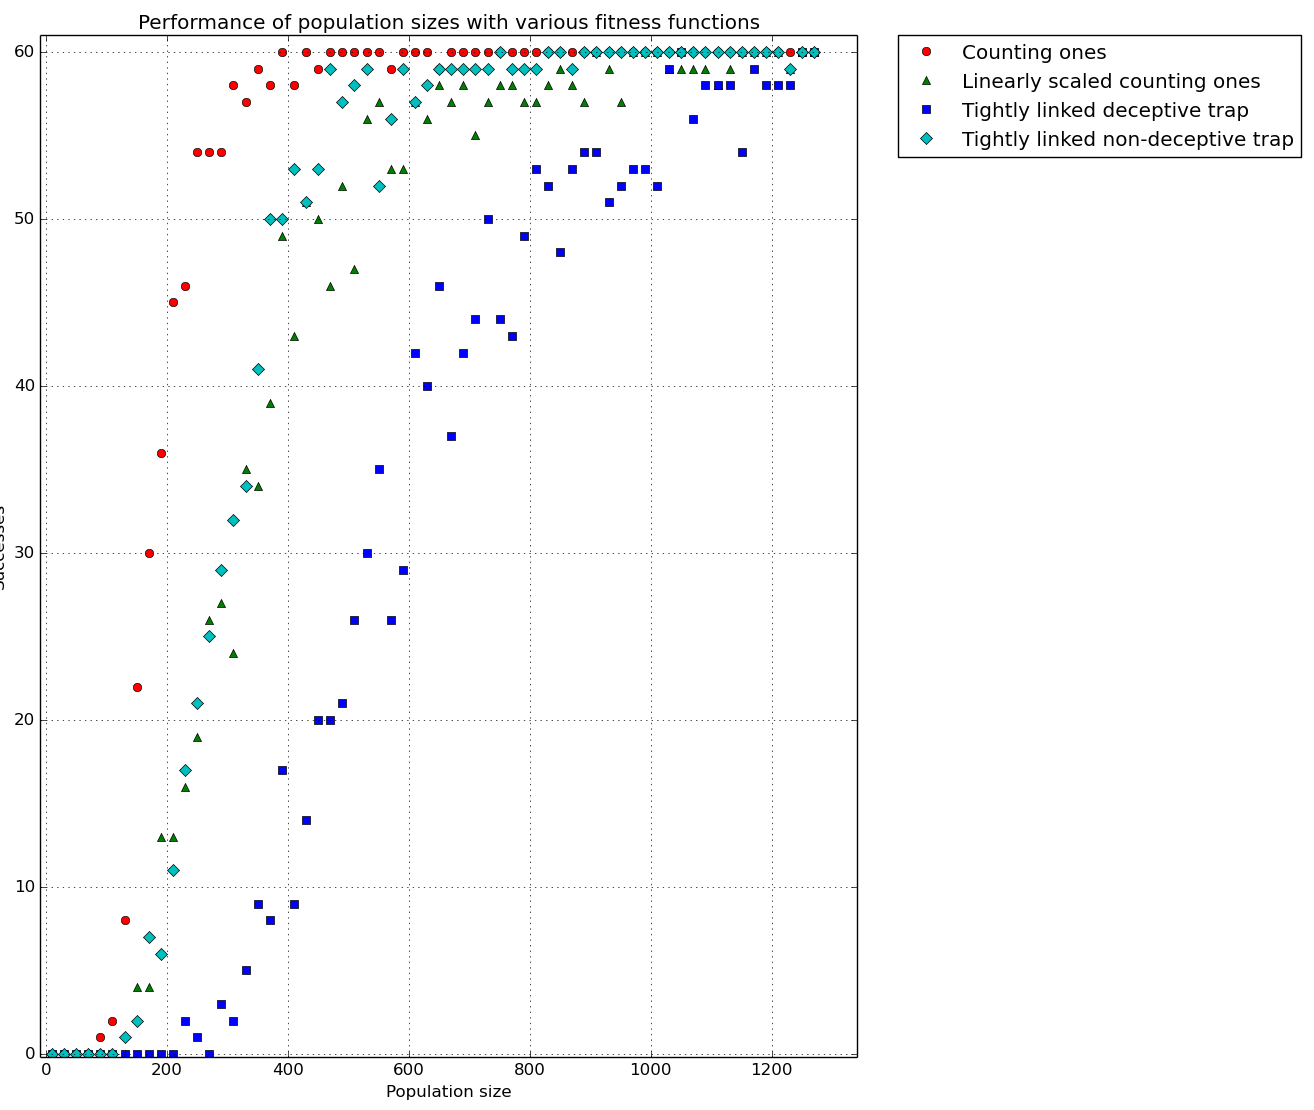
\includegraphics[totalheight=0.7\textheight]{images/exp1.png}
    \caption{Number of success per population size}
\label{fig:exp1}
\end{figure}

\begin{adjustwidth}{-1cm}{}
\begin{minipage}{\linewidth}
\centering
\captionof{table}{Table Title}
\label{tab:title}
\begin{tabular}{llll}
\toprule[1.5pt]
\bf Fitness function & \bf Population size & \bf Function evaluations & \bf CPU time\\\midrule
Counting ones & 310 & 51094 & 0.013 seconds \\
Linearly scaled Counting ones & 730 & 164174 & 0.030 seconds \\
Tightly linked deceptive trap & 1210 & 243142 & 0.429 seconds \\
Tightly linked non-deceptive trap & 610 & 93278 & 0.177 seconds \\
\bottomrule[1.25pt]
\end{tabular}\par
\bigskip
Should be a caption
\end{minipage}
\end{adjustwidth}


\subsection*{Experiment 2}
Tightly linked deceptive trap never reached an optimum.

\begin{figure}[H]
    \centering
    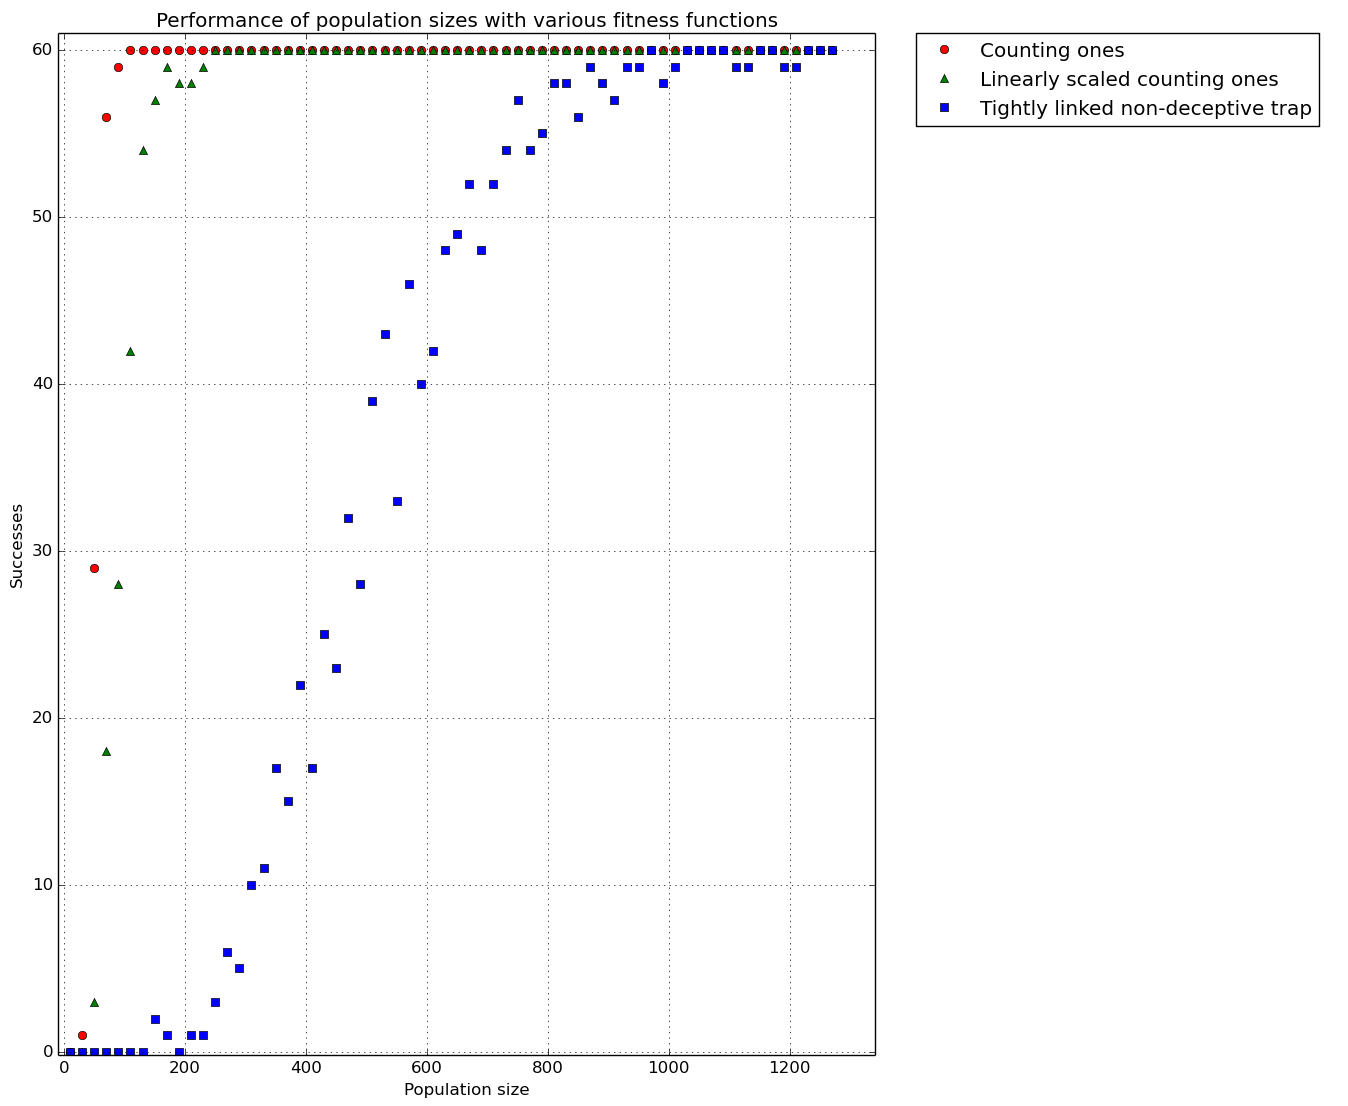
\includegraphics[totalheight=0.7\textheight]{images/exp2.png}
    \caption{Number of success per population size}
\label{fig:exp2}
\end{figure}

\begin{adjustwidth}{-1cm}{}
\begin{minipage}{\linewidth}
\centering
\captionof{table}{Table Title}
\label{tab:title}
\begin{tabular}{llll}
\toprule[1.5pt]
\bf Fitness function & \bf Population size & \bf Function evaluations & \bf CPU time\\\midrule
Counting ones & 70 & 9822 & 0.002 seconds \\
Linearly scaled Counting ones & 160 & 28260 & 0.005 seconds \\
Tightly linked non-deceptive trap & 850 & 242154 & 0.454 seconds \\
\bottomrule[1.25pt]
\end{tabular}\par
\bigskip
Should be a caption
\end{minipage}
\end{adjustwidth}


\subsection*{Experiment 3}
Tightly linked deceptive trap never reached an optimum.

\begin{figure}[H]
    \centering
    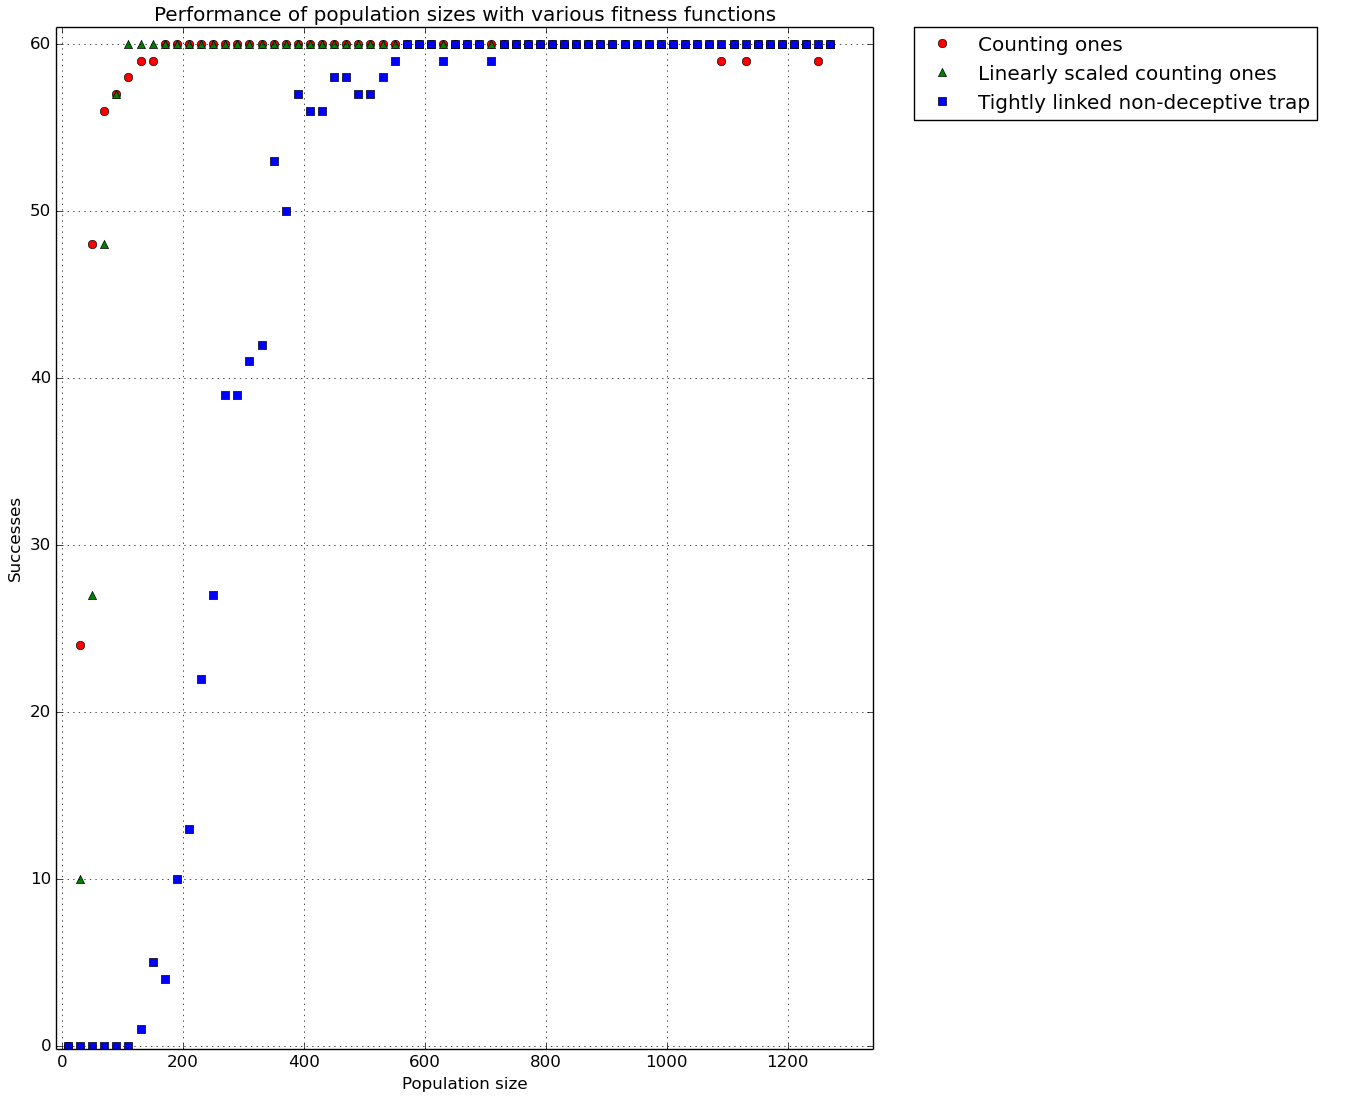
\includegraphics[totalheight=0.7\textheight]{images/exp3.png}
    \caption{Number of success per population size}
\label{fig:exp3}
\end{figure}

\begin{adjustwidth}{-1cm}{}
\begin{minipage}{\linewidth}
\centering
\captionof{table}{Table Title}
\label{tab:title}
\begin{tabular}{llll}
\toprule[1.5pt]
\bf Fitness function & \bf Population size & \bf Function evaluations & \bf CPU time\\\midrule
Counting ones & 110 & 27964 & 0.007 seconds \\
Linearly scaled Counting ones & 90 & 49764 & 0.010 seconds \\
Tightly linked non-deceptive trap & 490 & 509742 & 0.582 seconds \\
\bottomrule[1.25pt]
\end{tabular}\par
\bigskip
Should be a caption
\end{minipage}
\end{adjustwidth}



\section{Conclusions}



\begin{thebibliography}{9}

\bibitem{cython}
R. Bradshaw, S. Behnel, D. S. Seljebotn, G. Ewing, et al.,
The Cython compiler, \url{http://cython.org}.

\end{thebibliography}


\end{document}
